\BiChapter{环流的涨落定理}{Fluctuation theorems of cycle currents}

\BiSection{单环马氏链 LE 环流的涨落定理}{}
一个重要的问题是经验环流是否满足各种对称关系和涨落定理。LE经验环流的暂态涨落定理已经在文献 \cite{andrieux2007network} 中证明。这里将证明单环马氏链的对称关系,它甚至强于暂态涨落定理。记单环系统中两个 N 状态环为  $C^+ = (1,2,\cdots,N)$ 和 $C^- = (1,N,\cdots,2)$,令 $N^+_n$ 和 $N^-_n$ 分别表示 n 时刻环  $C^+$ 和 $C^-$ 分别形成的数量。强对称关系为:
\begin{align} \label{strong_symmetric}
    &\;k^+ \mathbb{P}\left(N^+_n=k^+,N^-_n=k^- -1,N^c_n=k^c,\;\forall c\neq C^+,C^-\right)\\
    =&\; \left(\frac{\gamma^+}{\gamma^-}\right)\mathbb{P}\left(N^+_n=k^+ -1,N^-_n=k^-,N^c_n=k^c,\;\forall c\neq C^+,C^-\right)\\
\end{align}
其中 $\gamma^+ = p_{12}p_{23}\cdots p_{N1}$ 和 $\gamma^- = p_{1N}p_{N,N-1}\cdots p_{21}$ 分别是环 $C^+$ 和环 $C^-$中的转移概率的乘积。对于序列匹配中得到的另一种环流,也可以得到类似的等式\cite{pietzonka2021cycle}。接下来。针对LE环流,证明\ref{strong_symmetric}。在周围边界条件下,由
公式 \eqref{trajectories} 可以得到:
\begin{align*}
    &\;\mathbb{P}\left(N^+_n=k^+,N^-_n=k^-,N^c_n=k^c,\;\forall c\neq C^+,C^-\right)\\
    =&\; (\gamma^+)^{k^+}(\gamma^-)^{k^-}\prod_{c\neq C^+,C^-}
    \left(\gamma^c\right)^{k^c}\left|G_n(k^+,k^-,(k^c)_{c\neq C^+,C^-})\right|,
\end{align*}
其中$G_n(k^+,k^-,(k^c)_{c\neq C^+,C^-})$ 表示n时刻所有容许轨迹的集合,那么 $C^+$ 形成 $k^+$ 次,$C^-$ 形成 $k^- -1$ 次,环 $c\neq C^+,C^-$ 形成 $k^c$ 次。简化记号,上述方程可以重写为:
\begin{equation}\label{temp1}
    \mathbb{P}\left(N^+_n=k^+,N^-_n=k^- -1,\cdots\right)
    = (\gamma^+)^{k^+}(\gamma^-)^{k^-}\prod_{c\neq C^+,C^-}\left(\gamma^c\right)^{k^c}|G_n(k^+,k^- -1,\cdots)|.
\end{equation}
类似地, 如果交换上式中的 $k^+$ 和 $k^- -1$,可以得到
\begin{equation}\label{temp2}
\mathbb{P}\left(N^+_n=k^+ -1,N^-_n=k^-,\cdots\right)
= (\gamma^+)^{k^+ -1}(\gamma^-)^{k^-}\prod_{c\neq C^+,C^-}\left(\gamma^c\right)^{k^c}|G_n(k^+ -1,k^-,\cdots)|.
\end{equation}
因此,为证明公式 \ref{strong_symmetric},只需说明:
\begin{equation} \label{equal0}
    k^+ |G_n(k^+, k^- -1, \cdots)| = k^-|G_n(k^+ -1,k^-,\cdots)|.
\end{equation}
% 文献 \cite{andrieux2007network} 中的证明是基于 $G_n(k^+,k^-,\cdots)$ 与 $G_n(k^-,k^+,\cdots)$ 之间的一一对应关系的,即

对于 $G_n(k^+,k^- -1,\cdots)$ 中的任意轨迹 $(\xi_0,\xi_1,\cdots,\xi_n)$,因为$C^+$形成$k^+$次,这个环有$k^+$个初始时刻和$k^+$个终止时刻。令$T_i^{begin}$和$T_i^{end}$分别表示环$C^+$的第$i$个初试时刻和第$i$个终止时刻。例如,表 \ref{trajectory}中的轨迹,环$(1,2,3,4)$的首次初始时刻是$n=0$,首次终止时刻是$n=7$。如果在$T_i^{begin}$和$T_i^{end}$之间翻转轨迹$\xi$,那么得到新轨迹$\tilde{\xi}$,即:
\begin{equation*}
    \tilde{\xi}
    =\left\{\begin{aligned}
        \xi_{T_i^{begin}+T_i^{end}-m},&   &&if ~ T_i^{begin} \le m \le T_i^{end}\\
        \xi_m, &   && \text{otherwise}.\\
        \end{aligned}\right.
\end{equation*}
易知,逆轨迹一定处于集合$G_n(k^+ -1,k^-,\cdots)$。因为环$C^+$形成$k^+$次,所以有$k^+|G_n(k^+,k^- -1, \cdots)|$种可能的轨迹。在这些逆轨迹中,$k^-$轨迹是完全相同的,因此被重复计算。例如,如果环$C^+=(1,2,3)$,那么$G_8(2,1,\cdots)$中的轨迹$\{1,2,3,1,2,3,1,3,2\}$和轨迹$\{1,2,3,1,3,2,1,2,3\}$都是$G_8(1,2,\cdots)$中$\{1,2,3,1,3,2,1,3,2\}$的逆轨迹,因此被计算两次。因此,$G_n(k^+ -1,k^-,\cdots)$的所有可能的轨迹数是:
\begin{equation}\label{equal}
    |G_n(k^+ -1,k^-,\cdots)| = \frac{k^+}{k^-}|G_n(k^+,k^- -1,\cdots)|.
\end{equation}
这恰好就是公式\ref{equal0}。因此已经证明了强对称关系\ref{strong_symmetric}。应用对称关系$|k^+ -k^-|$次,可以得到暂态涨落定理:
\begin{equation}\label{theorem:transient fluatuation}
	\mathbb{P}\left(N^+_n=k^+,N^-_n=k^-,\cdots\right)
	= \mathbb{P}\left(N^+_n=k^-,N^-_n=k^+,\cdots\right)\left(\frac{\gamma^+}{\gamma^-}\right)^{k^+-k^-}.
\end{equation}

% 对于 $G_n(k^+,k^- -1,\cdots)$ 中的任意轨迹 $(\xi_0,\xi_1,\cdots,\xi_n)$ 都可以在 $G_n(k^-,k^+,\cdots)$ 中找到对应的逆轨迹  $(\xi_n,\xi_{n-1},\cdots,\xi_0)$。也就是说轨迹中环 $C^+$ 形成 $k^+$ 次,环$C^-$ 形成 $k^-$ 次,相应的逆轨迹中环 $C^+$ 形成 $k^-$ 次,环$C^-$ 形成 $k^+$ 次。同时也可得到两个集合中的元素数量相同,即:
% \begin{equation}\label{equal}
%     |G_n(k^+,k^-,\cdots)| = |G_n(k^-,k^+,\cdots)|.
% \end{equation}
% 结合 \eqref{temp1},\eqref{temp2},和\eqref{equal},可以得到 LE 经验环流的暂态涨落定理:
目前,在周期边界条件下,已经证明了对称关系 \ref{strong_symmetric}和涨落定理 \ref{thm:transition fluatuation}。没有周期边界条件,两个等式在单环系统下也是成立的;证明过程类似,在此省略。

% 然而,上面也指出直观的想法是基于周期边界条件。例如,表\ref{example} 中的四状态单环系统的轨迹,其中环 $C^+$ 形成一次,然而相应的反环并没有形成$C^+$ 和 $C^-$。这说明逆轨迹并没有 $G_n(k^+,k^-,\cdots)$ 和 $G_n(k^-,k^+,\cdots)$ 之间的一一对应关系。
% % \begin{table}[htb!]
% % \renewcommand\arraystretch{1.3}\centering
% % \begin{tabular}{cccccccccc} \hline\hline
% % $n$                 & 0   & 1     & 2       & 3         & 4         & 5         & 6     & 7       \\ \hline
% % trajectory          & 1   & 2     & 3       & 4         & 4         & 1         & 4     & 3       \\ \hline
% % derived chain       & [1] & [1,2] & [1,2,3] & [1,2,3,4] & [1,2,3,4] & [1]       & [1,4] & [1,4,3] \\ \hline
% % cycles formed       &     &       &         &           & (4)       & (1,2,3,4) &       &         \\ \hline\hline
% % $n$                 & 0   & 1     & 2       & 3     & 4     & 5     & 6     & 7       \\ \hline
% % reversed trajectory & 3   & 4     & 1       & 4     & 4     & 3     & 2     & 1       \\ \hline
% % derived chain       & [3] & [3,4] & [3,4,1] & [3,4] & [3,4] & [3]   & [3,2] & [3,2,1] \\ \hline
% % cycles formed       &     &       &         & (1,4) & (4)   & (3,4) &       &         \\ \hline\hline
% % \end{tabular}
% % \caption{环擦除方式形成环的例子}\label{example}
% % \end{table}
% 通过上述论证,确实可以通过假设周期边界条件简化,简化论证。只是逆轨迹无法做到两个集合之间的一一映射,但这并不能否认暂态涨落定理 \eqref{theorem:transient fluatuation} 是错误的。在附录 E 中,给出了暂态涨落定理的严格证明。该证明的出发点是式 \eqref{trajectories} 中 $|G_n(k)|$ 的非平凡对称性。因为证明过于复杂,所以放在附录部分。这表明 LE 经验环流的联合分布满足一种非平凡对称性。

暂态涨落定理可以进用来其他两种涨落定理。回顾经验LE环流的矩母函数:
\begin{equation*}
    g_n(\lambda^+,\lambda^-,\cdots)
    = \mathbb{E}\left[e^{\lambda^+N^+_n+\lambda^-N^-_n+\sum_{c\neq C^+,C^-}\lambda^cN^c_n}\right].
\end{equation*}
可以得出 Kurchan-Lebowitz-Spohn 类型涨落定理成立:
\begin{align*}
    g_n(\lambda^+,\lambda^-,\cdots)
    &= \sum_{k}e^{\sum_{c\in\mathcal{C}}\lambda^ck^c}\mathbb{P}\left(N^+=k^+,N^-=k^-,\cdots\right)\\
    &= \sum_{k}e^{\sum_{c\in\mathcal{C}}\lambda^ck^c}
    \mathbb{P}\left(N^+=k^-,N^-=k^+,\cdots\right) \left(\frac{\gamma^+}{\gamma^-}\right)^{k^+-k^-}\\
    &= \sum_{k}e^{\left(\lambda^+-\log\frac{\gamma^+}{\gamma^-}\right)k^++
    \left(\lambda^--\log\frac{\gamma^-}{\gamma^+}\right)k^-+\cdots}\mathbb{P}(N^+=k^-,N^-=k^+,\cdots)\\
    &= \mathbb{E}\left[e^{\cdots+\left(\lambda^--\log\frac{\gamma^+}{\gamma^-}\right)N^+_n+
    \left(\lambda^++\log\frac{\gamma^+}{\gamma^-}\right)N^-_n}\right]\\
    &= g_n\left(\lambda^--\log\frac{\gamma^+}{\gamma^-},
    \lambda^++\log\frac{\gamma^+}{\gamma^-},\cdots\right),
\end{align*}
其中 $\log(\gamma^+/\gamma^-)$ 是环 $C^+$ 的匹配度。接下来,考虑单环系统的极限行为,当n趋于无穷是时,易知:
\begin{align*}
e^{-nI_J(\cdots,\nu^+,\nu^-)}
&\propto \mathbb{P}\left(J^+_n=\nu^+, J^-_n=\nu^-, \cdots\right)\\
&= \mathbb{P}\left(\cdots,J^+_n=\nu^-, J^-_n=\nu^+\right)
\left(\frac{\gamma^+}{\gamma^-}\right)^{n(\nu^+-\nu^-)}\\
&\propto e^{-n\left[I_J(\nu^-,\nu^+,\cdots)-\left(\log\frac{\gamma^+}{\gamma^-}\right)
(\nu^+-\nu^-)\right]}.
\end{align*}
这蕴含着下面 Gallavotti-Cohen 形式的涨落定理成立:
\begin{equation}\label{G-C type fluctuation}
    I_J(\cdots,\nu^+,\nu^-)=I_J(\cdots,\nu^-,\nu^+)-\left(\log\frac{\gamma^+}{\gamma^-}\right)(\nu^+-\nu^-).
\end{equation}

类似地,可以得到经验LE净环流的涨落定理。对于单环系统,只需关注环$C^+$经验LE净环流$\tilde{J}_n^+$。令$\tilde{g}_n(\lambda) = \mathbb{E}[e^{\lambda n\tilde{J}^+_n}]$ 为 $\tilde{J}^+_n$的矩母函数,$I_{\tilde{J}}(x)$为相应的速率函数。LE净环流满足的各种涨落定理在此列出。证明方式类似,在此省略。
1) 暂态涨落定理:
\begin{equation*}
\frac{\mathbb{P}(\tilde{J}^+_n=x)}{\mathbb{P}(\tilde{J}^+_n=-x)}
= \left(\frac{\gamma^+}{\gamma^-}\right)^{nx}.
\end{equation*}

2) Kurchan-Lebowitz-Spohn 类型涨落定理:
\begin{equation*}
\tilde{g}_n(\lambda)=\tilde{g}_n\left(-\left(\lambda+\log\frac{\gamma^+}{\gamma^-}\right)\right).
\end{equation*}

3)积分涨落定理 : 取 $\lambda = -\log \gamma^+/\gamma^-$ 带入上面方程可得
\begin{equation*}
\mathbb{E}\left[e^{\lambda n\tilde{J}^+_n}\right]=1.
\end{equation*}

4) Gallavotti-Cohen 类型涨落定理:
\begin{equation*}
\tilde{I}_J(x)=\tilde{I}_J(-x)-\left(\log\frac{\gamma^+}{\gamma^-}\right)x.
\end{equation*}

因此熵产生可以分解为LE净环流\cite{Seifert_2012}的和,上述结论可以用来证明熵产生的涨落定理。
% 最后考虑熵产生涨落和环流涨落之间的关系。回顾熵产生的定义 \cite{jiang2004mathematical}:
% \begin{equation*}
% 	W_n=\frac{1}{2}\sum_{c\in\mathcal{C}}\tilde{J}^c_n\log\frac{\gamma^c}{\gamma^{c-}}=\tilde{J}^+_n\log\frac{\gamma^+}{\gamma^-}.
% \end{equation*}
% 熵产生的暂态涨落定理可以整理为:
% \begin{equation*}
% 	\frac{\mathbb{P}(W_n=x)}{\mathbb{P}(W_n=-x)}
% 	= \frac{\mathbb{P}(\tilde{J}^+_n=x/(\log\frac{\gamma^+}{\gamma^-}))}{\mathbb{P}(\tilde{J}^-_n=-x/(\log\frac{\gamma^+}{\gamma^-}))} = e^{nx}.
% \end{equation*}
% 其他形式的涨落定理也有类似形式,在此省略。

\BiSection{一般马氏链 LE 环流的涨落定理}{}
目前,已经验证了单环系统中马氏链环流相关的涨落定理,自然会联想到这些结论是否会适用于一般的马氏链。再开始讨论之前,先回顾文献 \cite{jia2016cycle}中的定义。记 $c_1=(i_1,i_2,\cdots,i_s)$ 和 $c_2=(j_1,j_2,\cdots,j_r)$ 是两个环。如果 $s=r$ 且 $\{i_1,i_2,\cdots,i_s\}=\{j_1,j_2,\cdots,j_r\}$,则称环 $c_1$ 和环 $c_2$ 相似。
换句话说,如果两个环包含的状态完全一致,则称两个环相似。例如,下面六个环 $(1,2,3,4)$,$(1,2,4,3)$,$(1,3,2,4)$,$(1,3,4,2)$,$(1,4,2,3)$ 和 $(1,4,3,2)$,互为相似关系。根据这个定义,环任意 $c$ 和它的反环 $c^-$ 一定是相似的。

首先考虑 LE 经验环流 $(J^c_n)_{c\in\mathcal{C}}$,其中$J_n^c=N_n^c/n$。对于一般马氏链,如果环$c_1$和$c_2$相似,有下列的对称关系成立:
\begin{equation}\label{transient1}
    \frac{k^{c_1} \Pnum(N^{c_1}_n=k^{c_1},N^{c_2}_n=k^{c_2}-1,N^{c}_n=k^{c},\;\forall c\neq c_1,c_2)}
    {k^{c_2} \Pnum(N^{c_1}_n=k^{c_1} -1,N^{c_2}_n=k^{c_2},N^{c}_n=k^{c},\;\forall c\neq c_1,c_2)}
    = \frac{\gamma^{c_s}}{\gamma^{c_t}}.
\end{equation}
如果把环$c_1$和$c_2$分别设环$C^+$和它的反环$C^-$,那么等式可以化为:
\begin{equation*}
    \frac{k^{+} \Pnum(N^{+}_n=k^{+},N^{-}_n=k^{-}-1,N^{c}_n=k^{c},\;\forall c\neq C^+,C^-)}
    {k^{-} \Pnum(N^{+}_n=k^{+} -1,N^{-}_n=k^{-},N^{c}_n=k^{c},\;\forall c\neq C^+,C^-)}
    = \frac{\gamma^{c_s}}{\gamma^{c_t}}.
\end{equation*}
这可以被看做单环情况\ref{strong_symmetric}的一般化。重复使用\ref{transition1},可以给出下面LE环流的暂态涨落定理:
\begin{equation}\label{transient2}
    \frac{\Pnum(N^{c_1}_n=k^{c_1},N^{c_2}_n=k^{c_2},N^{c}_n=k^{c},\;\forall c\neq c_1,c_2)}
    {\Pnum(N^{c_1}_n=k^{c_2},N^{c_2}_n=k^{c_1},N^{c}_n=k^{c},\;\forall c\neq c_1,c_2)}
    = \left(\frac{\gamma^{c_1}}{\gamma^{c_t}}\right)^{k^{c_1}-k^{c_2}}.
\end{equation}
这表明如果环 $c_s$ 和环 $c_t$ 相似,那么 LE 经验环流的联合分布满足非平凡的对称关系。实际上,对于具有下面限制条件的情况,公式\ref{transient1}的证明已经在 \cite{jia2016cycle}中给出:1)所有环都通过状态$i\in S$;2)马氏链也是从状态$i$出发。
% 值得庆幸的是,这个假设条件可以移除,而且结论依然成立(整理中)


接下来考虑经验LE净环流$(\tilde{J}^{c}_n)_{c\in C}$。令$\{c_1,c_2,\cdots,c_r\}$表示所有环的集合,那么环$c$和它的反环$c^-$只出现一次,那么由\ref{transient2},可得:
\begin{align*}
    &\; \Pnum\left(\tilde{J}^{c_1}_n=x_1,\tilde{J}^{c_m}_n=x_m,\;\forall 2\le m \le r\right) \\
    =&\; \Pnum\left(N^{c_1}_n-N^{c_1-}_n=n x_1,N^{c_m}_n-N^{c_m-}_n=n x_m,\;\forall 2\le m \le r\right) \\
    =&\; \sum_{k^{c_i}-k^{c_i-}=n x_i,\forall 1\le i \le r} \Pnum\left(N^{c_1}_n=k^{c_1},N^{c_1-}_n=k^{c_1-},  N^{c_m}_n=k^{c_m},N^{c_m-}_n=k^{c_m-},\;\forall 2\le m \le r\right) \\
    =&\; \sum_{k^{c_i}-k^{c_i-}=n x_i,\forall 1\le i \le r} \Pnum\left(N^{c_1}_n=k^{c_1-},N^{c_1-}_n=k^{c_1}, N^{c_m}_n=k^{c_m},N^{c_m-}_n=k^{c_m-},\;\forall 2\le m \le r\right)\left(\frac{\gamma^{c_1}}{\gamma^{c_1-}}\right)^{n x_1}  \\
    =&\; \Pnum\left(N^{c_1}_n-N^{c_1-}_n=-n x_1, N^{c_m}_n-N^{c_m-}_n=n x_m,\;\forall 2\le m \le r\right) e^{n x_1 \log \frac{\gamma^{c_1}}{\gamma^{c_1-}}} \\
    =&\; \Pnum\left(\tilde{J}^{c_1}_n=-x_1,\tilde{J}^{c_m}_n=x_m,\;\forall 2\le m \le r\right) e^{n x_1 \log \frac{\gamma^{c_1}}{\gamma^{c_1-}}} .
\end{align*}
因此最终可得到下列的 LE 环流的暂态涨落定理:
\begin{equation}\label{strong}
    \Pnum(\tilde{J}^{c_1}_n=x_s,\tilde{J}^{c_m}_n=x_m,\;\forall 2\le m \le r) \\
    = \Pnum(\tilde{J}^{c_1}_n=-x_s,\tilde{J}^{c_m}_n=x_m,\;\forall 2\le m \le r)e^{nx_s\log\frac{\gamma^{c_1}}{\gamma^{c_1-}}}.
\end{equation}
这表明对于任意环$c_i$,经验LE净环流满足对称关系。如果对所有$1\le i \le r$,在上述方程中交换$x_i$和$-x_i$,那么可以得到:
\begin{equation}\label{weak}
    \begin{split}
    \frac{\Pnum\left(\tilde{J}^{c_1}_n=x_1,\tilde{J}^{c_2}_n=x_2,\cdots,\tilde{J}^{c_{r}}_n=x_{r}\right)}
    {\Pnum\left(\tilde{J}^{c_1}_n=-x_1,\tilde{J}^{c_2}_n=-x_2,\cdots,\tilde{J}^{c_{r}}_n=-x_{r}\right)}
    =e^{n\sum_{i=1}^{r}x_i\log\frac{\gamma^{c_i}}{\gamma^{c_i-}}}.
    \end{split}
\end{equation}
通过对比,可以看到\eqref{weak}式的结论弱于 \eqref{strong}式。因此,本文称 \eqref{strong} 式为强形式的暂态涨落定理,\eqref{weak}式为弱形式的暂态涨落定理。

有关 LE 经验环流和 LE 经验净环流的其他类型涨落定理都可以通过暂态涨落定理得到。这里主要关注强形式;弱形式也可以通过类似的方式得到。令$g_n(\lambda) = \mathbb{E}[e^{n\sum_{i=1}^r\lambda_i J^{c_i}_n}]$和$\tilde{g}_n(\lambda) = \mathbb{E}[e^{n\sum_{i=1}^{r}\lambda_i\tilde{J}^{c_i}_n}]$ 分别为 $(J^{c_i}_n)_{1\le i\le r}$ 和 $(\tilde{J}^{c_i}_n)_{1\le i\le r}$ 的矩母函数,并且令 $I_{J}(x)$ 和 $I_{\tilde{J}}(x)$ 为相应的速率函数。

1)Kurchan-Lebowitz-Spohn 类型涨落定理:对任意相似的两个环 $c_s$ 和 $c_t$ ($1\le s,t\le r$),下列公式成立:
\begin{equation*}
	g_n(\cdots,\lambda_s,\cdots,\lambda_t,\cdots) = g_n\left(\cdots,\lambda_t-\log\frac{\gamma^{c_s}}{\gamma^{c_t}},\cdots,\lambda_s+\log\frac{\gamma^{c_s}}{\gamma^{c_t}},\cdots\right).
\end{equation*}
\begin{equation*}
	\tilde{g}_n(\cdots,\lambda_s,\cdots)=\tilde{g}_n\left(\cdots,-\left(\lambda_s+\log\frac{\gamma^{c_s}}{\gamma^{c_s-}}\right),\cdots\right).
\end{equation*}

2)积分涨落定理,对任意子集$\{c_1,c_2,\cdots, c_t\} \subset \{c_1,c_2,\cdots, c_r\}$,有: 
\begin{equation*}
	\mathbb{E}\left[e^{-n\sum_{i=1}^t(\log \gamma^{c_i}/\gamma^{c_i-})\tilde{J}^{c_i}_n}\right]=1.
\end{equation*}

3)Gallavotti-Cohen 类型涨落定理,$c_s$ 和 $c_t$相似,则有:
\begin{equation*}
	I_J(\cdots,x_s,\cdots,x_t,\cdots)=I_J(\cdots,x_t,\cdots,x_s,\cdots)-\left(\log\frac{\gamma^{c_s}}{\gamma^{c_t}}\right)(x_s-x_t).
\end{equation*}
\begin{equation*}
	I_{\tilde{J}}(\cdots,x_s,\cdots) = I_{\tilde{J}}(\cdots,-x_s,\cdots)-\left(\log\frac{\gamma^{c_s}}{\gamma^{c_s-}}\right)x_s.
\end{equation*}

% \BiSection{单环马氏链 ST 环流的涨落定理}
\BiSection{一般马氏链 ST 环流的涨落定理}
现已经清楚了 LE 经验环流和 LE 经验净环流满足的各种涨落定理。自然会想到是否 ST 经验环流和 ST 经验净环流是否也满足类似的关系。事实上,所有的涨落定理对于经验ST环流都是不成立的,即使考虑单环系统。考虑全连接三状态马氏链,并且令 $T = 1\to 2\to 3$ 是一个生成树,那么相应基本集为$\mathcal{L} = \{(1),(2),(3),(1,2),(2,3),(1,2,3),(1,3,2)\}.$回顾式 \eqref{formula:I_Q} 中的 ST 经验环流的速率函数为:
\begin{equation*}
I_Q(\mu) = \sum_{\langle i,j\rangle\in E}R^{\mu}(i,j)\log\frac{R^{\mu}(i,j)}{R^{\mu}(i)p_{ij}},
\end{equation*}
其中 $R^{\mu}(i,j)=\sum_{c_l\in\mathcal{L}}\mu^{c_l}H^{c_l}(i,j)$ 且 $R^{\mu}(i)=\sum_{j\in S}R^{\mu}(i,j)$。再记 $\mu^+ = \mu^{(1,2,3)}$ , $\mu^- = \mu^{(1,3,2)}$。图\ref{figure:ratefunction}(a)说明的是在一组适当参数下,$I_Q(\cdots,\mu^+,\mu^-)$和$I_Q(\cdots,\mu^-,\mu^+)-\log(\gamma^+ /\gamma^-) (\mu^+-\mu^-)$之间的差异,易知两者相差不是0,因此有:
\begin{equation*}
I_Q(\cdots,\mu^+,\mu^-)
\neq I_Q(\cdots,\mu^-,\mu^+)-\left(\log\frac{\gamma^+}{\gamma^-}\right)(\mu^+-\mu^-),
\end{equation*}
这说明了 Gallavotti-Cohen 类型涨落定理对于 ST 环流不成立。且由于Gallavotti-Cohen 类型涨落定理成立条件最弱,所以其他类型涨落定理也不成立。
\begin{figure}[h]
	\centering
	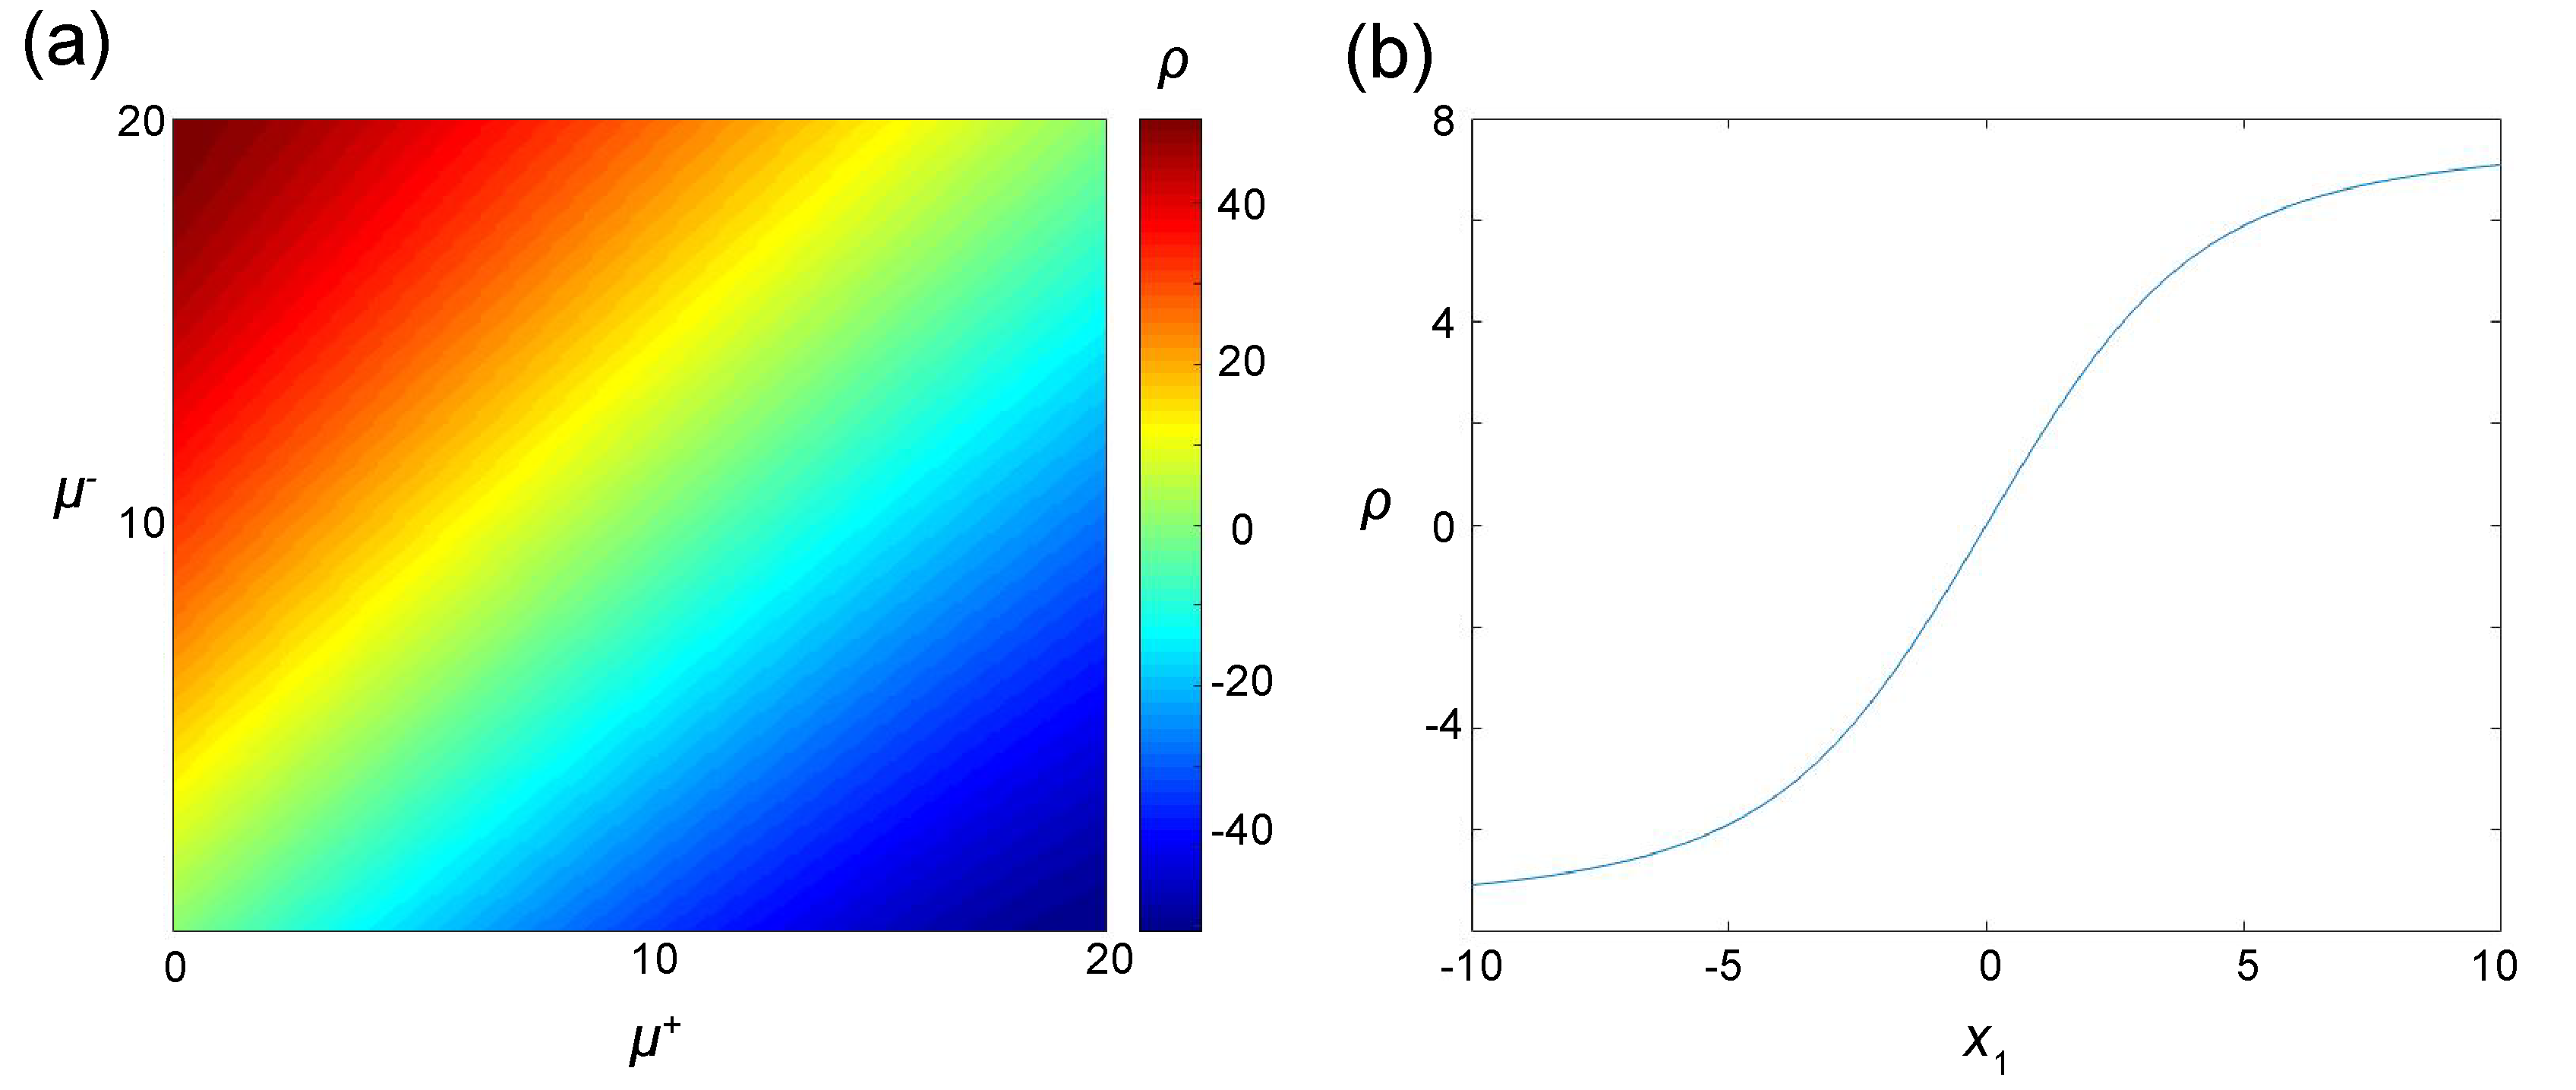
\includegraphics[scale=0.25]{chart/ratefunction.pdf}
	\caption{ST 经验环流和经验净环流的速率函数图像 (a) $\rho=I_Q(\cdots,\mu^+,\mu^-)-I_Q(\cdots,\mu^-,\mu^+)+(\log\frac{\gamma^+}{\gamma^-})(\mu^+-\mu^-)$. (b) $\rho=I_{\tilde{Q}}(\tilde{\mu}^{c_1},\tilde{\mu}^{c_2},\tilde{\mu}^{c_3})- I_{\tilde{Q}}(-\tilde{\mu}^{c_1},\tilde{\mu}^{c_2},\tilde{\mu}^{c_3})
		+(\log\frac{\gamma^{c_1}}{\gamma^{c_1-}})\tilde{\mu}^{c_1}$}\label{figure:ratefunction}
\end{figure}
尽管 ST 经验环流无法满足各种涨落定理,ST 经验净环流在很多情况下成立却是可以的(参考 \cite{andrieux2007fluctuation})。
%%%%%%%%%%%%%%%%%%%%%%%%%%%%%%%%%%%%%%%%%%%%%%%%%%%%%%%%%%%%






对于单环系统,只需考虑环 $C^+$ 的净环流。从 \eqref{conversion} 式中易知环 $C^+$ 的 ST 经验净环流  $\tilde{Q}^+_n$ 等于 该环的 LE 经验净环流 $\tilde{J}^+_n$。记弦 $l^+$ 和 $l^-$ 分别对应于 $C^+$ 和 $C^-$,由于 $l^+=l^--$,则:
\begin{equation*}\label{circulation}
    \begin{split}
            \tilde{Q}^{+}_n =&\;\sum_{c\in \mathcal{C}}J^c_n1_{\{l^+\in c \}}-\sum_{c\in \mathcal{C}}J^c_n1_{\{l^-\in c \}}\\
            =&\;\sum_{c\in \mathcal{C}}J^c_n1_{\{l^+\in c \}}-\sum_{c\in \mathcal{C}}J^{c-}_n1_{\{l^+\in c \}} = \tilde{J}^+_n.
    \end{split}
\end{equation*}
因此 ST 净环流的涨落定理自然等同于 LE 环流的涨落定理。然而,\eqref{conversion} 式只在周期边界条件下成立,也就意味着,只能得到 ST 经验净环流满足 Gallavotti-Cohen 类型涨落定理。并且,容易验证 $\tilde{Q}^+_n$ 对其他三种类型涨落定理不成立。


\BiSection{一般马氏链的 ST 环流的涨落定理}{}

关于单环马氏系统,ST 经验环流无法满足各种涨落定理,然而 ST 经验净环流满足 Gallavotti-Cohen 类型涨落定理。对于一般情形的马氏链,Andrieux 和 Gaspard 在文献 \cite{andrieux2007fluctuation} 中已经证实了 ST 经验净环流满足弱形式下的 Gallavotti-Cohen 类型涨落定理:对于基本集 $\mathcal{L}$ 中三状态以上的环  $c_1,c_1-,c_2,c_2-,\cdots,c_r,c_r-$,满足:
\begin{equation*}
I_{\tilde{Q}}(x_1,x_2,\cdots,x_r)
= I_{\tilde{Q}}(-x_1,-x_2,\cdots,-x_r)
-\sum_{i=1}^rx_i\log\frac{\gamma^{c_i}}{\gamma^{c_i-}}.
\end{equation*}
这表明 ST 经验净环流的联合分布具有对称性。

更加让人难以置信的是,对比 LE 经验净环流,可以发现 ST 经验净环流不满足强形式下的 Gallavotti-Cohen 类型涨落定理。下面将通过举出反例证实。考虑图 \ref{figure:transitiongraph}(b) 中的具有全连接转移图的四状态马氏链,并且令生成树为 $T=1\to2\to3\to4$。由于对所有一状态和两状态的环 $c_l$,有 $\tilde{Q}^{c_l}_n=0$,因此只考虑其余的环:
\begin{equation*}
	c_1 = (1,2,3),\;c_2 = (2,3,4),\;c_3 = (1,2,3,4),\;c_4 = (1,3,2),\;
	c_5 = (2,4,3),\;c_6 = (1,4,3,2).
\end{equation*}
注意到所有三状态以上的环满足 $\tilde{Q}^{c_l}_n=-\tilde{Q}^{c_l-}_n$ 且 $c_1=c_4-$, $c_2=c_5-$, $c_3=c_6-$。回顾 ST 经验环流的速率函数,可知 $(\tilde{Q}^{c_1}_n,\tilde{Q}^{c_2}_n,\tilde{Q}^{c_3}_n)$ 的速率函数为:
\begin{equation*}
	I_{\tilde{Q}}(x)=\inf_{\{\mu\in\mathcal{M}:\mu^{c_i}-\mu^{c_i-}= x_i,\forall 1\le i\le 3\}}I_Q(\mu).
\end{equation*}
对于环 $c_1$,如果把 $\tilde{\mu}^{c_1}$ 换为 $-\tilde{\mu}^{c_1}$,那么有图 \ref{figure:ratefunction} (b) 可以得到:
\begin{equation*}
I_{\tilde{Q}}(\tilde{\mu}^{c_1},\tilde{\mu}^{c_2},\tilde{\mu}^{c_3})\neq I_{\tilde{Q}}(-\tilde{\mu}^{c_1},\tilde{\mu}^{c_2},\tilde{\mu}^{c_3})
-\left(\log\frac{\gamma^{c_1}}{\gamma^{c_1-}}\right)\tilde{\mu}^{c_1},
\end{equation*}
这表明 ST 经验净环流不满足 Gallavotti-Cohen 类型涨落定理的强形式。